\documentclass[11pt,english]{report}

\usepackage{siunitx}
\sisetup{range-phrase={ -- }}
\sisetup{range-units=single}
\usepackage{amsmath}
\newcommand\numberthis{\addtocounter{equation}{1}\tag{\theequation}}
\usepackage{amssymb}

\usepackage{mathspec}
\setallmonofonts[
  AutoFakeSlant,
  BoldItalicFeatures={FakeSlant},
  ]{Inconsolata}

\usepackage{polyglossia}
\usepackage{microtype}

\usepackage{float}
\usepackage{graphicx}
\usepackage[hypcap]{caption}
\graphicspath{ {pics/} }


\usepackage{perpage}
\MakePerPage{footnote}

\usepackage{tikz}
\usetikzlibrary{shapes,arrows}
\tikzstyle{block} = [draw, rectangle, minimum height=3em, minimum width=6em]
\tikzstyle{square} = [draw, rectangle, minimum height=3em, minimum width=3em]
\tikzstyle{sum} = [draw, circle, node distance=1cm]
\tikzstyle{input} = [coordinate]
\tikzstyle{output} = [coordinate]
\tikzstyle{pinstyle} = [pin edge={to-,thin,black}]

\usepackage{todonotes}

\usepackage{placeins}

\usepackage{booktabs}

\usepackage{minted}
\newminted{matlab}{
  frame=lines,
  framesep=2mm,
  fontsize=\tiny,
  mathescape
}

\usepackage{xcolor}
\definecolor{link}{HTML}{4078C0}
\usepackage[colorlinks=true, allcolors = black, linktoc = all]{hyperref}

\setcounter{tocdepth}{1}


\begin{document}
\pagenumbering{roman}
\begin{titlepage}
\centering

\topskip0pt
\vspace*{\fill}


\includegraphics[width=0.4\textwidth]{bruface.jpg}~\\ [0.75cm]
{\Large CSD Labs Technical Report}\\ [0.3cm]
{\Large Control of a Rolling Mill}\\[0.7cm]

{\large Nathan \textsc{Dwek} -- Thomas \textsc{Lapauw}}\\[0.2cm]

{\small \today}

\vspace{5cm}
\vspace*{\fill}

\end{titlepage}

\setcounter{page}{2}
{\small
\tableofcontents}

\hypersetup{allcolors = link}
\chapter{Introduction}
\pagenumbering{arabic}
\section{Description of the plant}
The goal of this project is to control the rolling of a metallic strip using a rolling mill. The plant is composed of two DC motor driven single rolls which unwind and wind up the sheet of metal. Between those two, the strip passes through a pair of rolls driven by a third DC motor, in order to have its thickness reduced and made uniform.

The actuators of the plant are the three DC motors, which are controlled through their armature current. The speed of those motors are measured using three velocity sensors. There are also two traction sensors to measure the tension in the strip left and right of the middle pair of rolls. Finally, a thickness sensor measures the thickness of the metallic strip after it has been rolled.

The first requirement is to control the traction of the metallic strip. When this is achieved, a more advanced requirement is to control the thickness of the metallic strip.

\section{Broad design of the controller}
The plant will be controlled using a numerical controller implemented in matlab. To set this up, eight ADC and two DAC ports are available, along with second order Butterworth filters with various $\tau$ and an analog computer.

Intuitively, we know that the traction of the strip between two rolls will probably mostly depend on the difference of speed between the rolls. Similarly, we also know that the thickness reduction at the middle pair of rolls will probably mostly depend on the difference between the traction of the strip that is fed into the pair of rolls and the traction of the sheet that is pulled out of it. Knowing this, we propose to control this process using a cascade controller.

First, we control the speed of the DC motors using the current as input. Then, we control the traction of the metallic strip using the speed of the motors as input. Finally, we control the thickness of the metallic sheet using the tractions of the strips as input.

Moreover, since we know that the traction will depend on a \emph{difference} of speeds, we also propose to simplify this scheme by modulating the speed of only one motor during the operation. One motor will be designated as ``master'': it will be controlled with a constant reference with the only goal of spinning at the setpoint speed as steadily as possible. The other will be designated as ``slave'': its reference will vary during operation in order to control the traction of the strip and it should have adequate transient response properties.

\section{Structure of this report}
This report will follow the chronological order of the work that was done during the labs. We used a bottom up approach where the inner loops are first implemented in order to then design the outer loops.

As stated before, to simplify the controller, only one motor -- the slave -- is controlled with a dynamic reference while the other -- the master -- is kept at a as steady as possible. In chapter \ref{chap:master} \todo{reference}, the dynamics of the master motor are identified and a controller is designed to achieve zero steady state error and perturbation rejection. Then, in chapter \ref{chap:slave} \todo{reference}, the dynamics of the slave motor are identified and a controller is designed to achieve reasonably fast reference tracking.

In chapter \ref{chap:traction} \todo{reference}, the relation between both motors' speed and the traction of the metallic strip is modelled and identified, and a controller is designed to stabilize the system and reduce the steady state error.

Finally, ... \todo{What comes next?}






\chapter{Description of the Experimental Setup}
\label{chap:setup}
\section{General Wiring}
The setup is wired as described in figure \ref{fig:wiring}.
\begin{figure}[htbp]
\centering
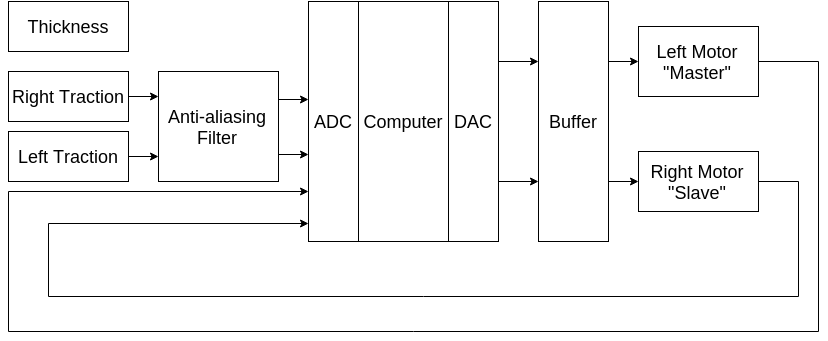
\includegraphics[width = \textwidth]{wiring.png}
\caption{\label{fig:wiring}Wiring for the control of the rolling mill}
\end{figure}
We use the maximum recommended sampling frequency $f_s  = \SI{100}{\hertz}$, which is a common value for the control of a DC motor.

\subsection{Anti-aliasing filtering}
To be perfectly rigorous, we should filter every input before sampling it. However, we only have a limited amount of single signal, second order Butterworth filters at our disposition, each with a different $f_c$. With the chosen $f_s$, those constraints on the available $f_c$, and the fact that second order Butterworth filters have a large transition band, only two of the available $f_c$ values seem actually useful:
\begin{itemize}
 \item $f_c = \SI{40}{\hertz}$, which provides \SI{37.1}{\percent} attenuation at \SI{50}{\hertz} and \SI{62.9}{\percent} rejection at \SI{100}{\hertz}.
 \item $f_c = \SI{20}{\hertz}$, which provides \SI{62.9}{\percent} attenuation at \SI{50}{\hertz} and \SI{80.4}{\percent} rejection at \SI{100}{\hertz}.
\end{itemize}

The other available filters either do not actually prevent aliasing, or have a too high passband attenuation. Even the two most adequate filters have a non ideal passband gain, and thus introduce a significant delay in the feedback loop. For this reason we choose not to use them in the inner loop, which should be fast, but rather in the outer loop. This is why only the two traction measurements are filtered in figure \ref{fig:wiring}.


\chapter{Control of the Master Motor}
\label{chap:masterMotor}
In this chapter, we will identify and design a controller for the master motor of the rolling mill. During the operation, this motor will be controlled with a constant reference and it should keep its velocity as steady as possible.

\section{Master motor}
The master motor is the one that pulls the strip and winds it up on a spool. The left motor was chosen as master since its setpoint velocity is higher than that of the right motor. This is necessary since when the strip is compressed to reduce its thickness it extends, which means the speed of the winding motor should be higher than the feeding motor. Figure \ref{fig:LM_RPM_curr} shows the static characteristic of the left motor and table \ref{tab:LM_operating_region} shows the currents and speed for different operating points.

\begin{figure}[htbp]
\centering
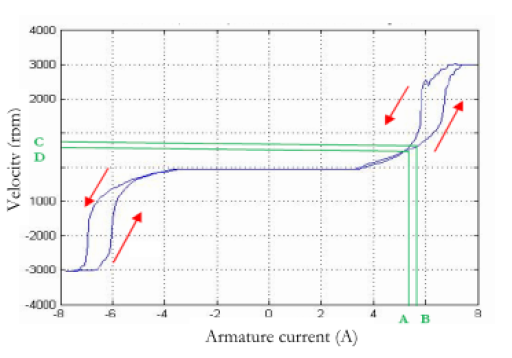
\includegraphics[width = .6\textwidth]{pics/LM_RPM_Current.png}
\caption{Static characteristic of the left motor\label{fig:LM_RPM_curr}}
\end{figure}

\begin{table}[htbp]
	\centering
	\begin{tabular}{rr}
    \toprule
		Armature current [A] & Angular velocity [RPM] \\ \midrule
    5.4 & 530.7 \\
    5.7 & 649.8 \\\bottomrule
	\end{tabular}
	\caption{Operating points of the left motor\label{tab:LM_operating_region}}
\end{table}

\section{Identification of the Transfer Function}
The transfer function of the left motor is identified with a least square approximation using matlab. To do this, the measured velocity is sampled for an input step between the setpoints, since that is the region where we want to linearize the behaviour of the motor. We choose to fit the system with a first order transfer function which is common for a DC motor with big inertial load.

Figure \ref{fig:LM_id} shows the measured and fitted step responses. We see that the system is indeed heavily dominated by a single slow real pole, and that it is well approximated by transfer function \ref{eq:LM_TF}.

\begin{equation}
	LM(s) = \frac{5.398}{3.642S+1}
  \label{eq:LM_TF}
\end{equation}

\begin{figure}[htbp]
\centering
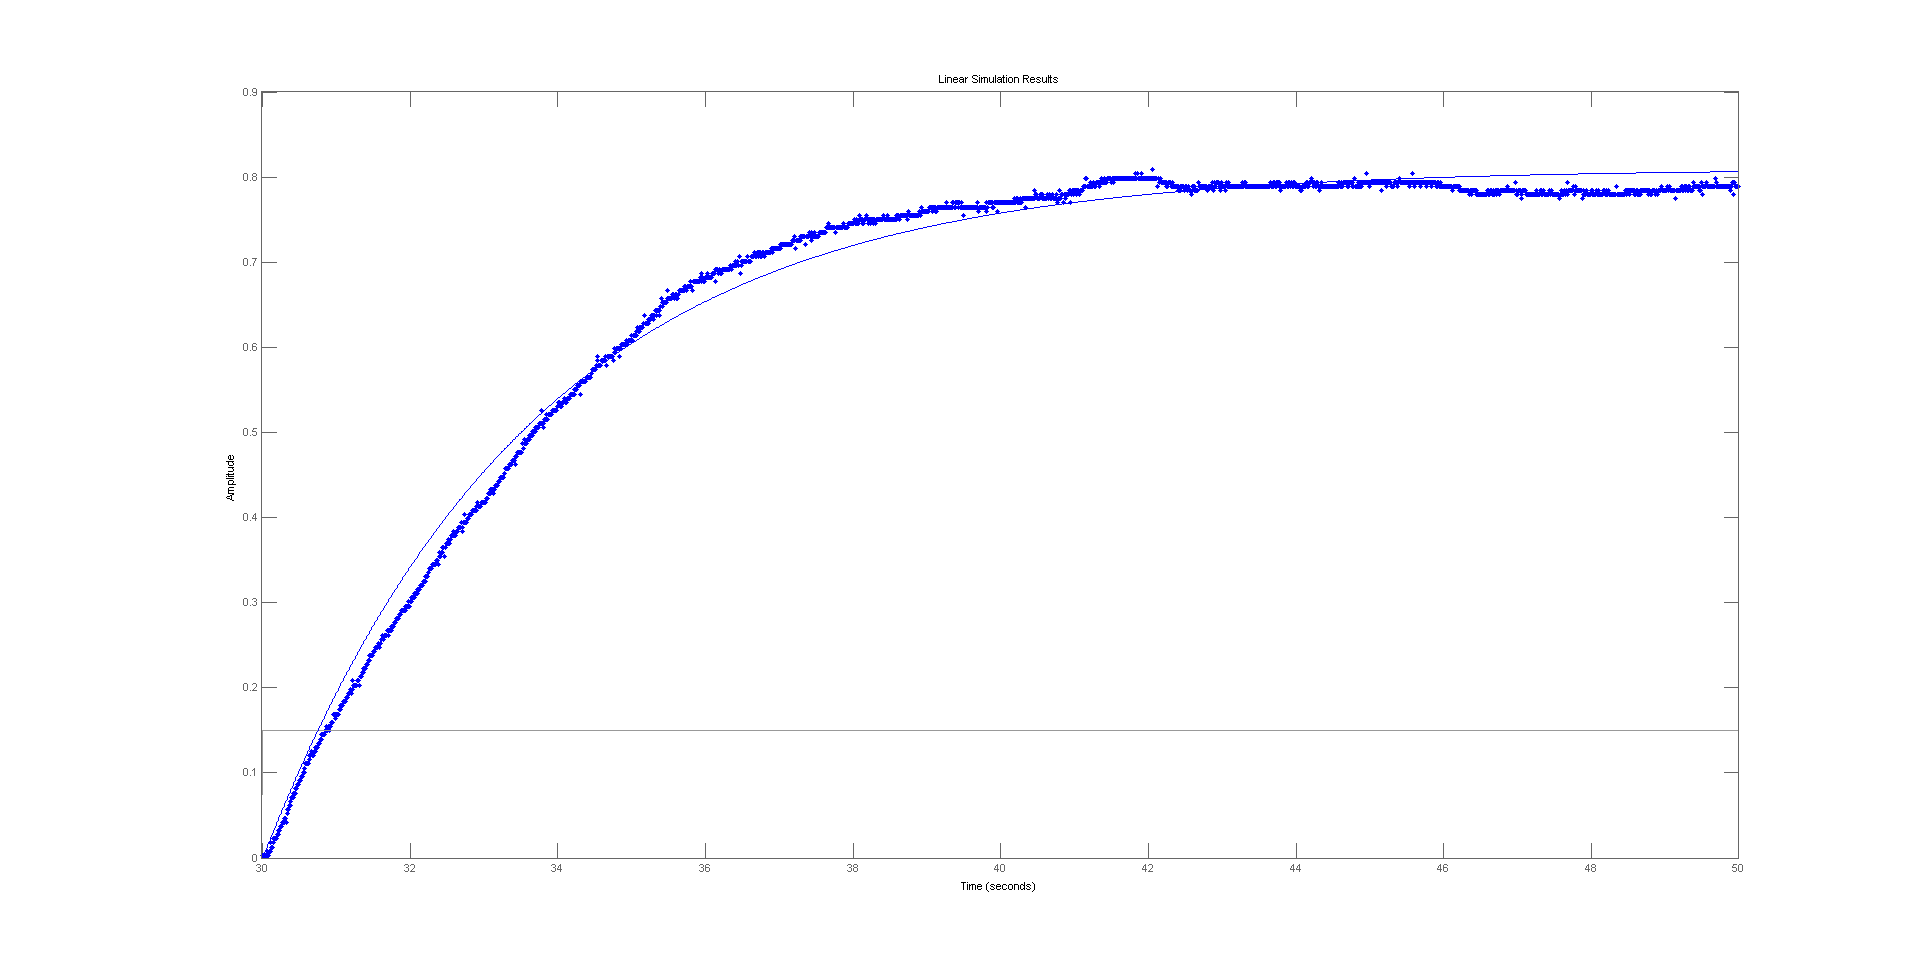
\includegraphics[width = \textwidth]{identification_step_setpoints.png}
\caption{Sampled and fitted step response of the left motor\label{fig:LM_id}}
\end{figure}

\section{Design of a PI Controller}
The master motor is controlled with a constant reference and should keep its velocity as steady as possible despite possible disturbance. For this reason, we choose to control it with a PI controller, which should provide asymptotic stability, zero steady state error, and perturbation rejection.

We use the root locus method to tune the PI controller. First we choose $\frac{K_I}{K_P}$ so that the zero of the controller cancels the pole of the motor. This theoretically ensures that the closed loop has a single negative real pole that can then be arbitrarily placed by adjusting $K_P$. In the following, we detail the calculations used to determine the gains using this method.

First, the transfer functions of the left motor and the PI controller are transformed to make the poles and zeroes immediately visible.
\begin{align*}
	LM(s) &= \frac{5.398}{3.642s+1}\\
				&= \frac{1.482}{s+0.274}\\
\\PI(s) &= K_p + \frac{K_i}{s}\\
    		&= K_p \cdot \frac{s+\frac{K_i}{K_p}}{s}
\end{align*}
To cancel the pole of the motor, we hence use $\frac{K_i}{K_p} = 0.294$.

We then choose $K_P$ using a root locus. The open loop is given by:
\begin{align*}
    OL(s) &= \frac{1.482}{s+0.274} \cdot \frac{s+0.274}{s} \\
					&= \frac{1.482}{s}
\end{align*}

Figure \ref{fig:LM_rl}
\begin{figure}[htbp]
\centering
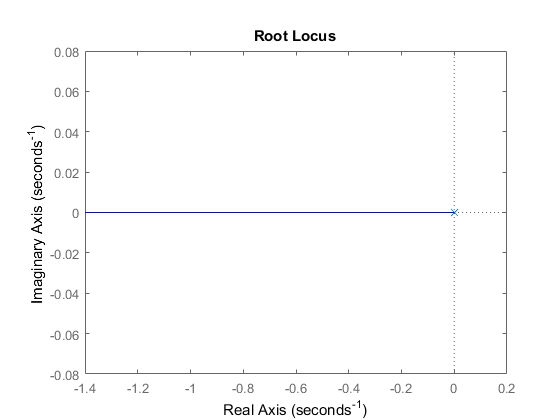
\includegraphics[width = .7\textwidth]{pics/LM_cont_rlocus.png}
\caption{Root locus plot for the left motor with a PI controller\label{fig:LM_rl}}
\end{figure}
shows that $K_P > 0$ can theoretically be chosen arbitrarily. Non linearities, higher order effects and actuator saturation will determine its ideal value.

Figures \ref{fig:LM_SIM_KP050} -- \ref{fig:LM_SIM_KP200}
\begin{figure}[htbp]
\centering
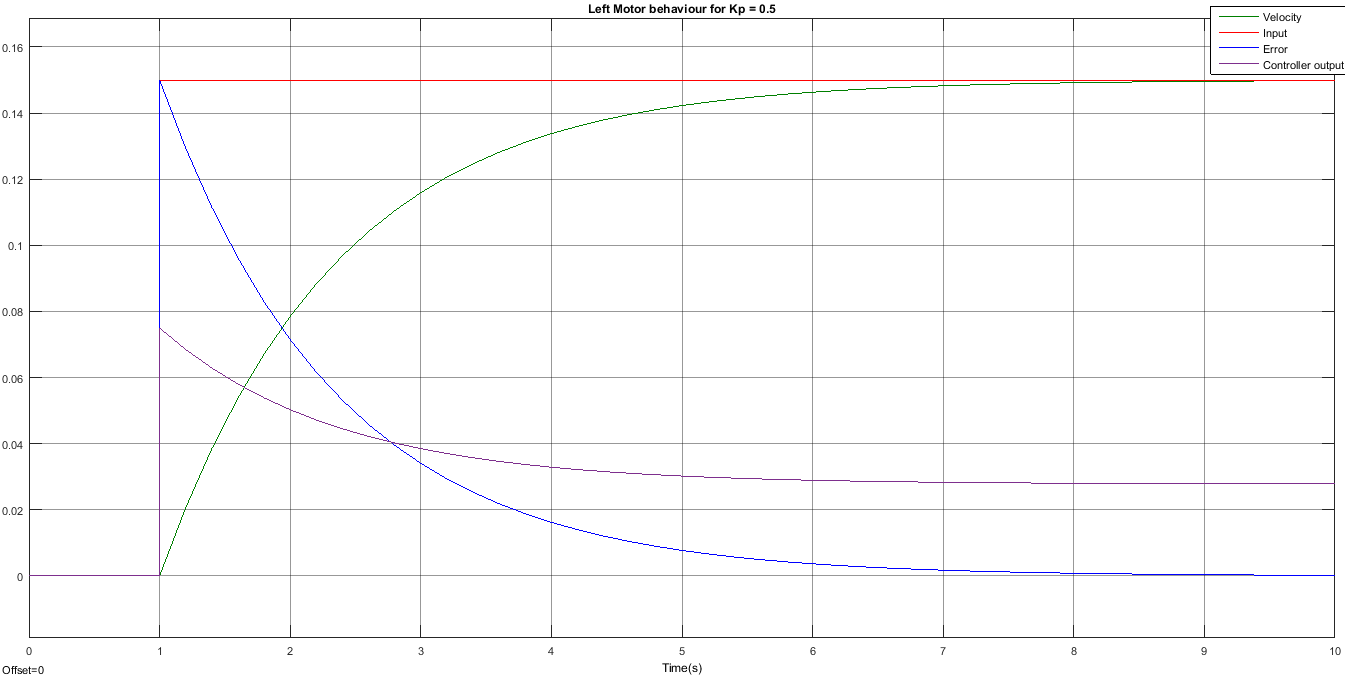
\includegraphics[width = \textwidth]{pics/LM_KP050_Sim.png}
\caption{Simulink simulation of the left motor behaviour for $K_p = 0.5$}
\label{fig:LM_SIM_KP050}
\end{figure}
%
\begin{figure}[htbp]
\centering
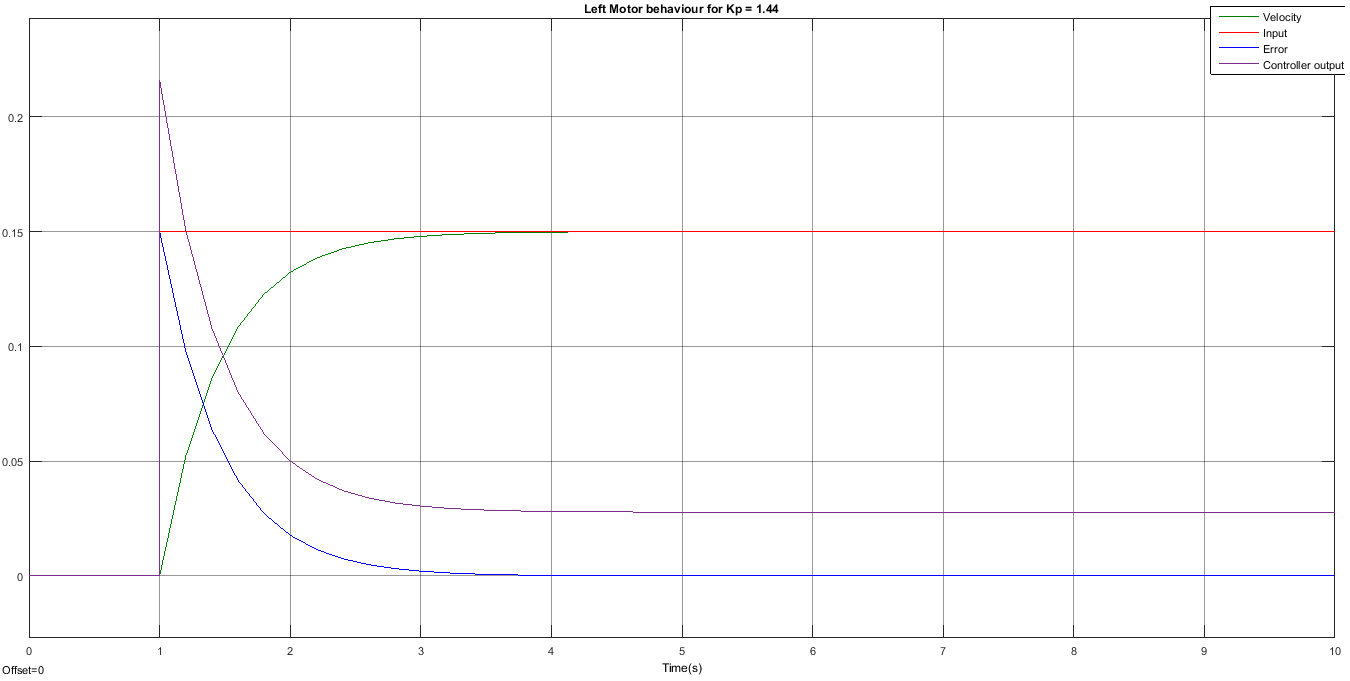
\includegraphics[width = \textwidth]{pics/LM_KP144_Sim.png}
\caption{Simulink simulation of the left motor behaviour for $K_p = 1.44$}
\label{fig:LM_SIM_KP144}
\end{figure}
%
\begin{figure}[htbp]
\centering
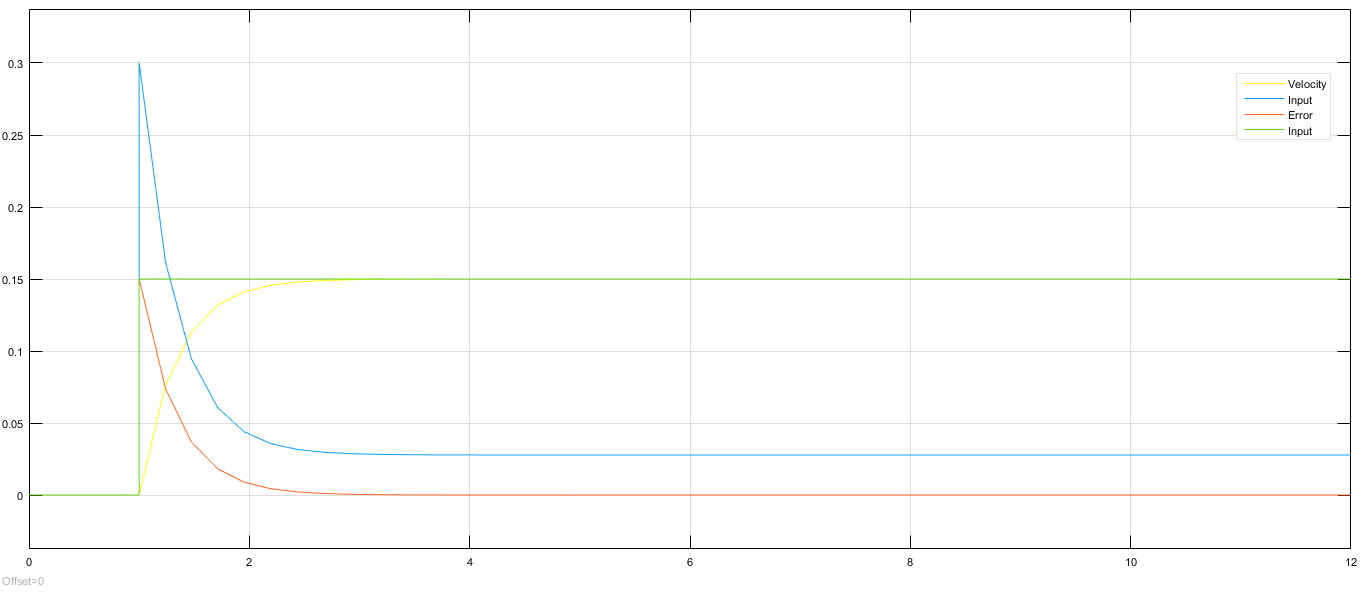
\includegraphics[width = \textwidth]{pics/LM_KP200_sim.png}
\caption{Simulink simulation of the left motor behaviour for $K_p = 2$}
\label{fig:LM_SIM_KP200}
\end{figure}
show the result of simulink simulations for several values of $K_P$. We see that actuator saturation will probably not be the deciding constraint\footnote{The blue curve represents the small signal input on each of the plots. The setpoint value is \SI{2.7}{V} and the input range is [\SI{-10}{V} - \SI{10}{V}].}. We thus need to implement the controller to be able to experimentally tune its gain.

\FloatBarrier
\section{Tuning of the PI Controller}
Figures \ref{fig:LM_KP050} -- \ref{fig:LM_KP200} show experimental runs of the master motor with different values of $K_P$. Based on these measurements $K_P = 1.44$ was chosen. $K_P = 0.5$ has a longer settling time with a larger overshoot than $K_p = 1.44$, and $K_P = 0.5$ has a longer, higher overshoot.  Since $\frac{K_I}{K_P} = 0.294$, $K_I = 0.3954$. None of the simulations have overshoot while all the practical experiments do. This is because the transfer function of the motor was reduced to a first order system while in practice it behaves as a non linear system of higher order.
\begin{figure}[htbp]
\centering
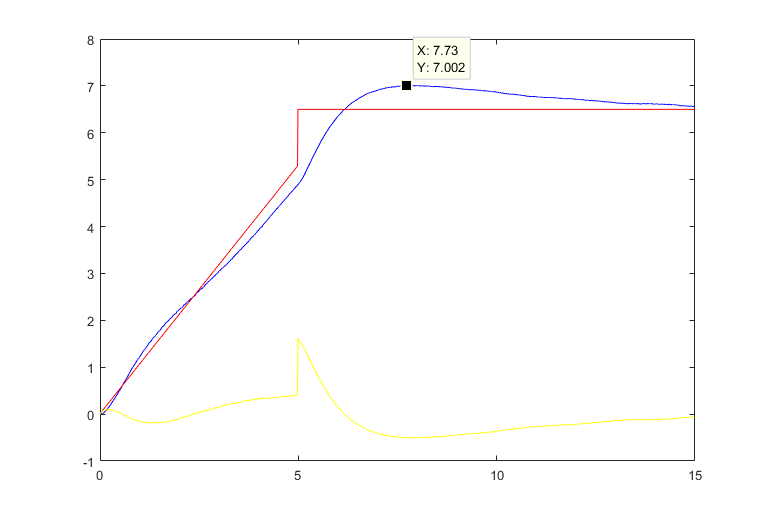
\includegraphics[width = .7\textwidth]{pics/LM_KP050a.png}
\caption{Response of the left motor behaviour for $K_p = 0.5$ to the red curve as input.}
\label{fig:LM_KP050}
\end{figure}
%
\begin{figure}[htbp]
\centering
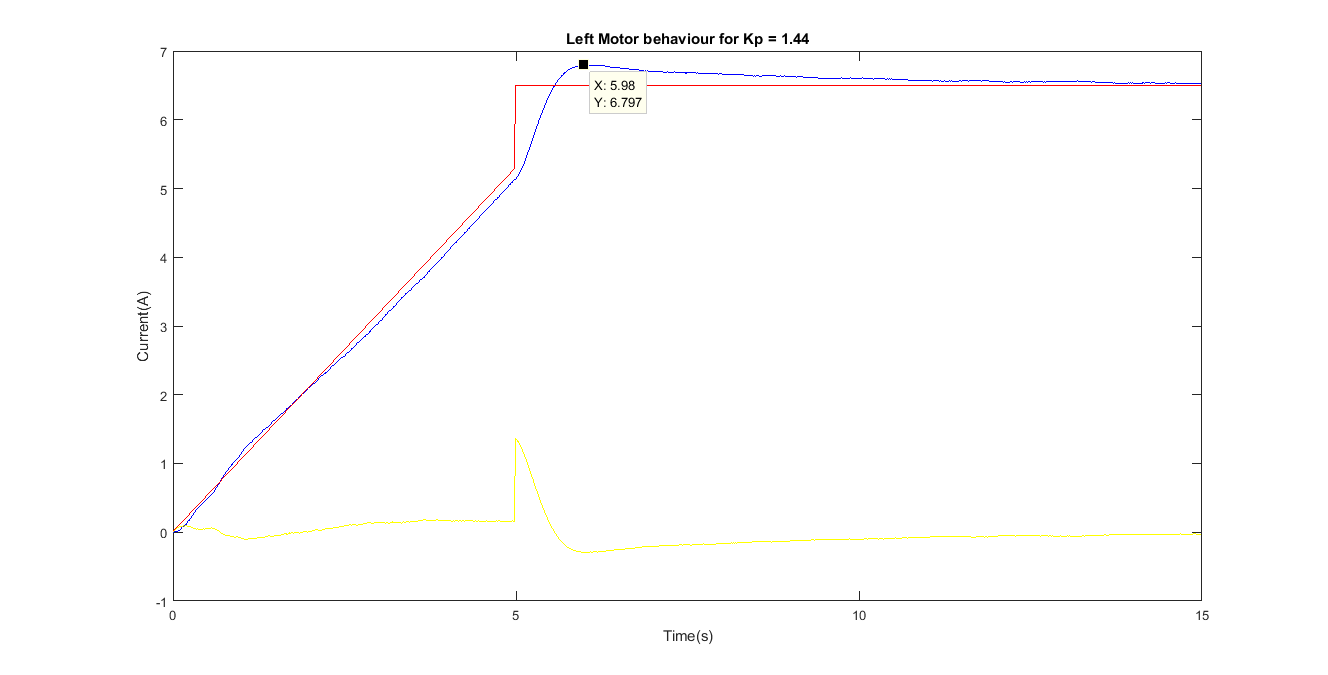
\includegraphics[width = \textwidth]{pics/LM_KP144.png}
\caption{Response of the left motor behaviour for $K_p = 1.44$ to the red curve as input.}
\label{fig:LM_KP144}
\end{figure}
%
\begin{figure}[htbp]
\centering
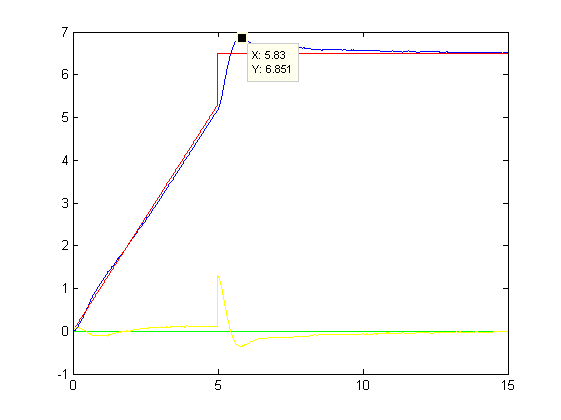
\includegraphics[width = .7\textwidth]{pics/LM_KP200.png}
\caption{Response of the left motor behaviour for $K_p = 2$ to the red curve as input.}
\label{fig:LM_KP200}
\end{figure}

We observe that we indeed obtain zero steady state error, and that disturbances of order higher than 1 seem to not affect the master velocity too much, which is very good.
\section{Conclusion}
We decide to control the master motor with a PI controller and the following values:
\begin{align*}
	K_P = 1.44
	K_I = 0.3954
\end{align*}
This allows us to generate a steady, precise master speed around which we will then modulate the slave speed in order to control the traction of the metallic strip. In the next chapter, we will identify and design a controller for the slave motor, which will serve as an inner loop for the traction control.


\chapter{Control of the Slave Motor}
\label{chap:slaveMotor}
In this chapter the properties of the design of the controller for the slave motor will be explained. The process is analogous to the master motor, first the motor is identified around the operating point, then a controller is designed which is then simulated and tested in practice.

\section{Slave motor}

Now that the master motor has a controller to keep the speed constant the slave motor can be controlled. The slave motor feeds the metal strip to the master motor. The right motor will be the slave. The speed of the feeding motor has to be lower than the winding motor. Figure \ref{fig:RM_RPM_curr} shows a plot of the motor characteristics and table \ref{tab:RM_operating_region} shows the currents for different operating points.

\begin{figure}[htbp]
\centering
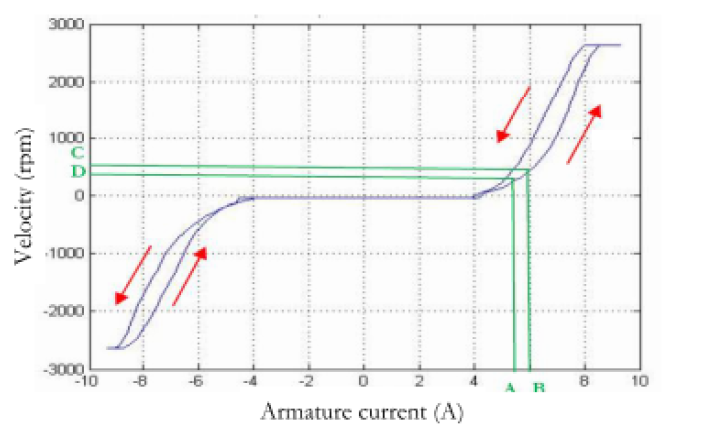
\includegraphics[width = .7\textwidth]{pics/RM_RPM_Current.png}
\caption{Rotational Velocity of the Right motor in function of the Current}
\label{fig:RM_RPM_curr}
\end{figure}

\begin{table}[H]
	\centering
		\begin{tabular}{c|c}
        \toprule
			Armature current [A] & Angular velocity [RPM] \\ \midrule
            5.4 & 244 \\
            5.7 & 370 \\
		\end{tabular}
	\caption{Operating points of the right motor}
	\label{tab:RM_operating_region}
\end{table}

\FloatBarrier

\section{Identifying the transfer function}
The transfer function was identified the same way the master motor was done: stepping from one operating point to another and measuring the step response. Using the least squares method a best fitting curve (figure \ref{fig:RM_id}) to the sampled data points was generated with a corresponding first order transfer function (equation \ref{eq:RM_TF}). 

\begin{align}
	G(s) = \frac{7.128}{6.0665S+1}
    \label{eq:RM_TF}
\end{align}

\begin{figure}[htbp]
\centering
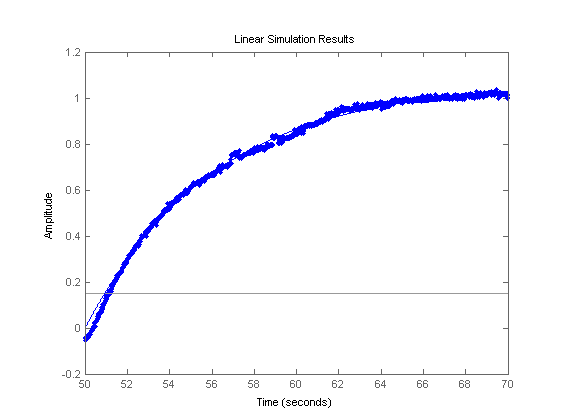
\includegraphics[width = 0.7\textwidth]{pics/RM_systemID.png}
\caption{Sampled data with the fitted curve from the calculated transfer function}
\label{fig:RM_id}
\end{figure}

\FloatBarrier
\section{Controller Design}
The controller for this motor needs to be fast enough to be able to keep the tension of the strip constant despite disturbances. To do this a proportional controller with gain $K$ was chosen. A proportional controller has a steady state error, but in this case this is negligible because this controller is part of a larger cascade controller.

Figure \ref{fig:RM_rlocus} shows a root locus plot for the right motor. The gain can again be chosen arbitrarily.$K$ was chosen based on a couple simulations (figures \ref{fig:RM_K2_SIM}, \ref{fig:RM_K3_SIM} and \ref{fig:RM_K4_SIM}) and  practical experiments for different gains (figures \ref{fig:RM_K2}, \ref{fig:RM_K3} and \ref{fig:RM_K4}). None of the simulations have overshoot while some of the practical experiments do (depending on $K$). This is because the transfer function of the motor was reduced to a first order system while in practice it probably as a non-linear system.

\begin{figure}[htbp]
\centering
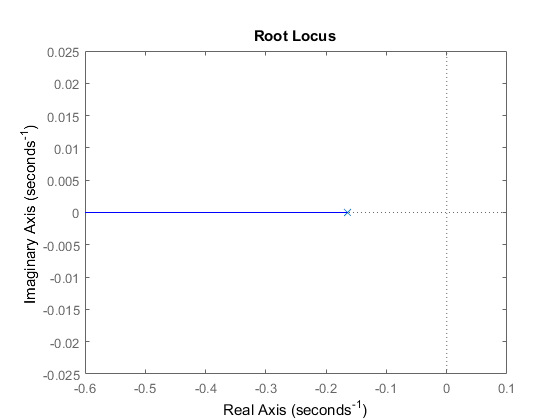
\includegraphics[width = \textwidth]{pics/RM_rlocus.png}
\caption{Root locus plot for the right motor}
\label{fig:RM_rlocus}
\end{figure}



A gain of $K = 3$ was used since using a higher gain has the risk of putting current output of the controller in saturation. Saturation will occur is a too large step is applied to the input of the controller, but in practice it should not occur. The system is started up using a ramp instead of using a step, but this will be explained in a later chapter.

\begin{figure}[htbp]
\centering
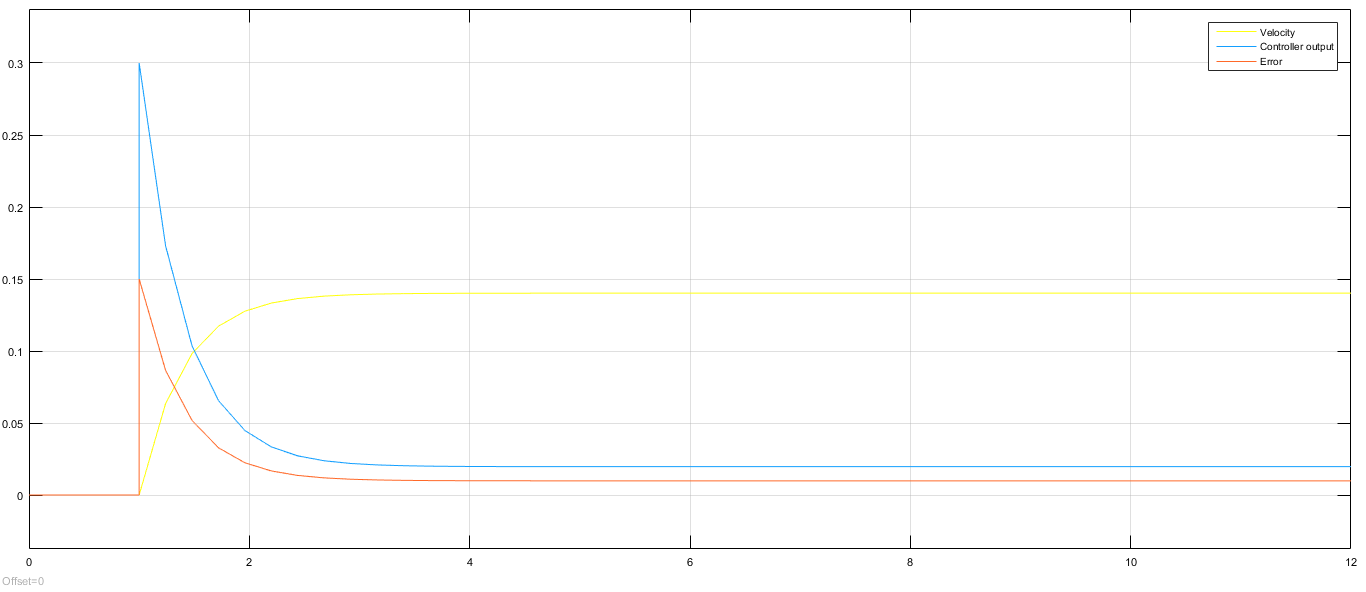
\includegraphics[width = \textwidth]{pics/RM_K2_SIM.png}
\caption{Simulink simulation of the right motor behaviour for $K = 2$}
\label{fig:RM_K2_SIM}
\end{figure}

\begin{figure}[htbp]
\centering
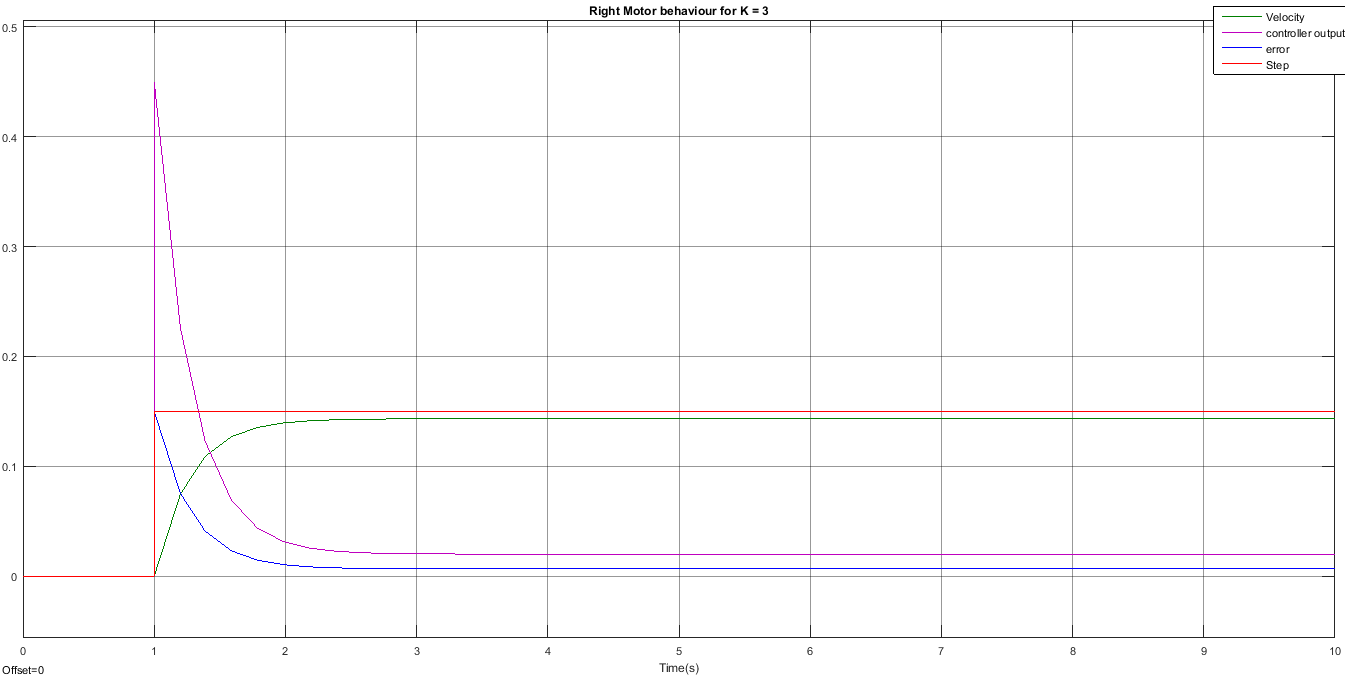
\includegraphics[width = \textwidth]{pics/RM_K3_SIM.png}
\caption{Simulink simulation of the right motor behaviour for $K = 3$}
\label{fig:RM_K3_SIM}
\end{figure}

\begin{figure}[htbp]
\centering
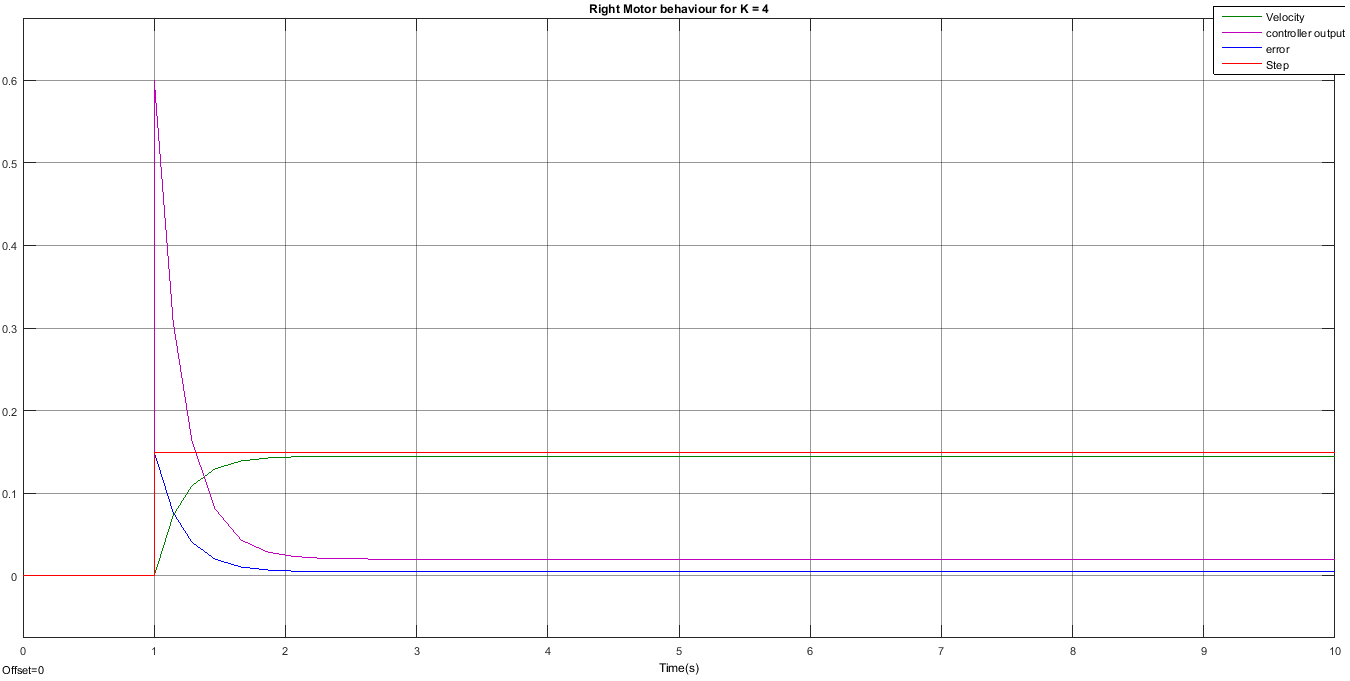
\includegraphics[width = \textwidth]{pics/RM_K4_SIM.png}
\caption{Simulink simulation of the right motor behaviour for $K = 4$}
\label{fig:RM_K4_SIM}
\end{figure}



\begin{figure}[htbp]
\centering
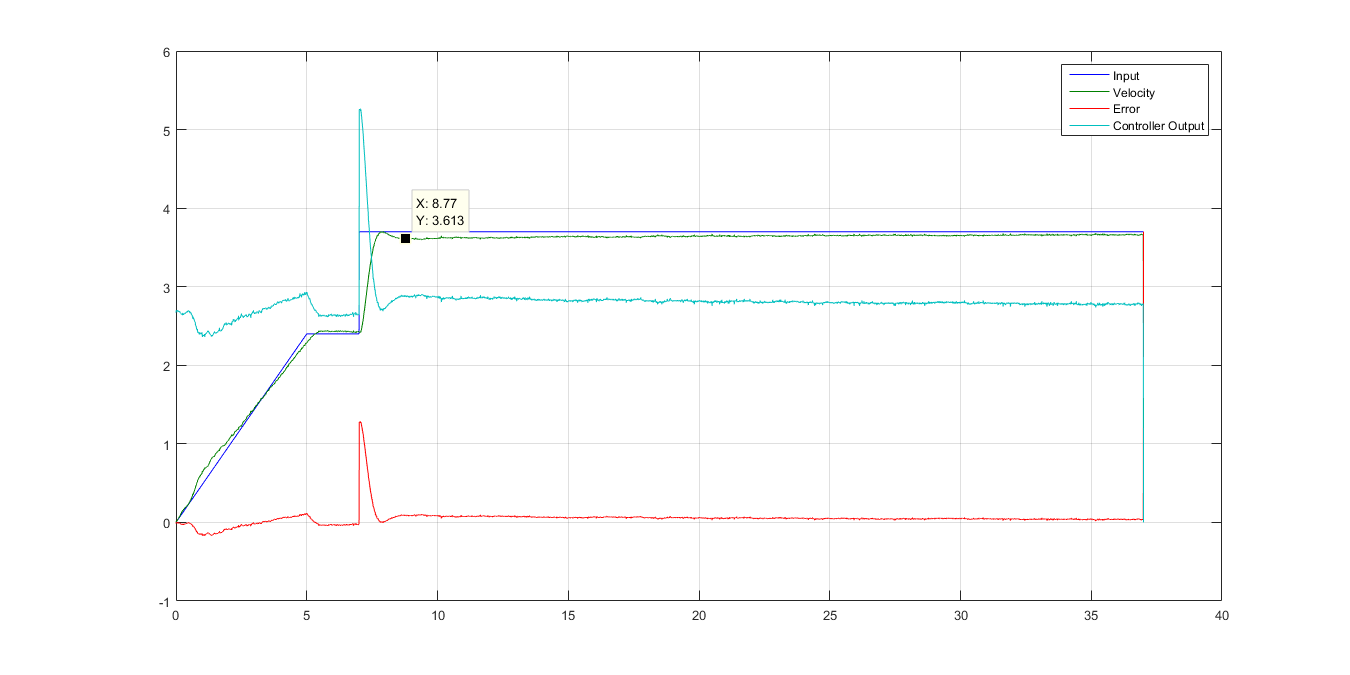
\includegraphics[width = \textwidth]{pics/RM_K2.png}
\caption{Response of the left motor behaviour for $K = 2$ to the blue curve as input.}
\label{fig:RM_K2}
\end{figure}

\begin{figure}[htbp]
\centering
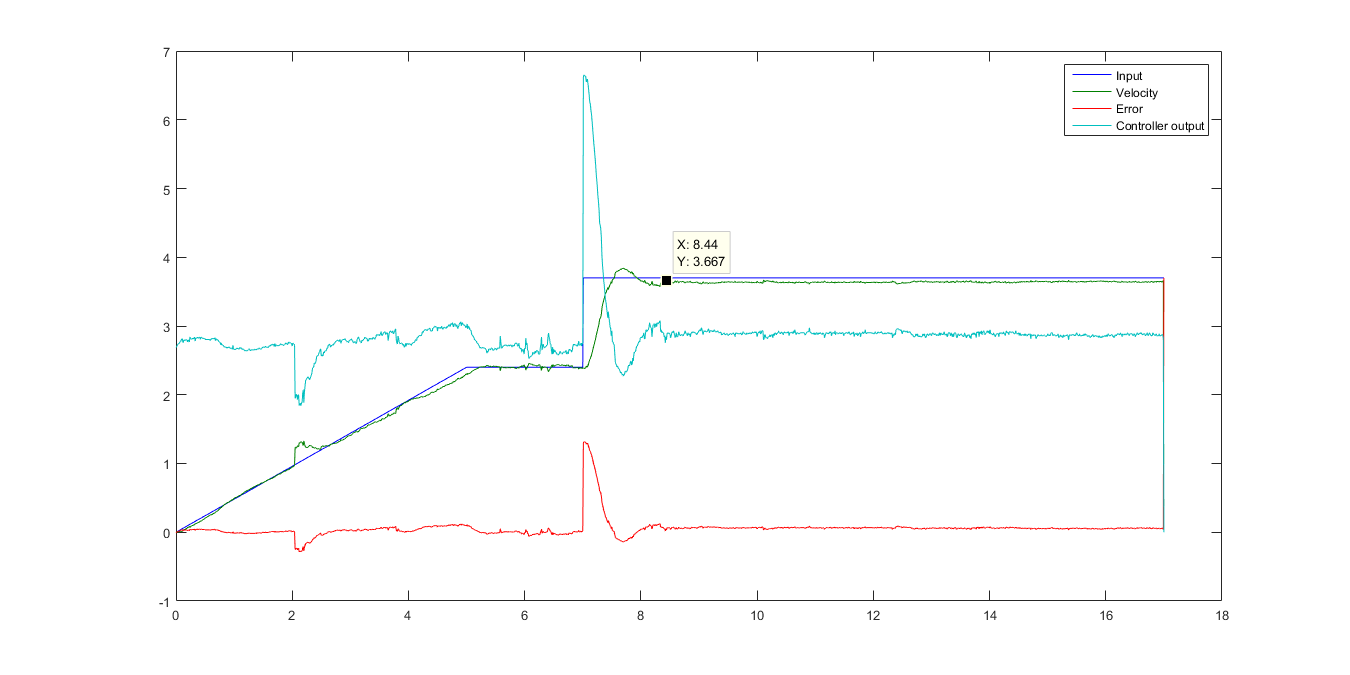
\includegraphics[width = \textwidth]{pics/RM_K3.png}
\caption{Response of the left motor behaviour for $K = 3$ to the blue curve as input.}
\label{fig:RM_K3}
\end{figure}

\begin{figure}[htbp]
\centering
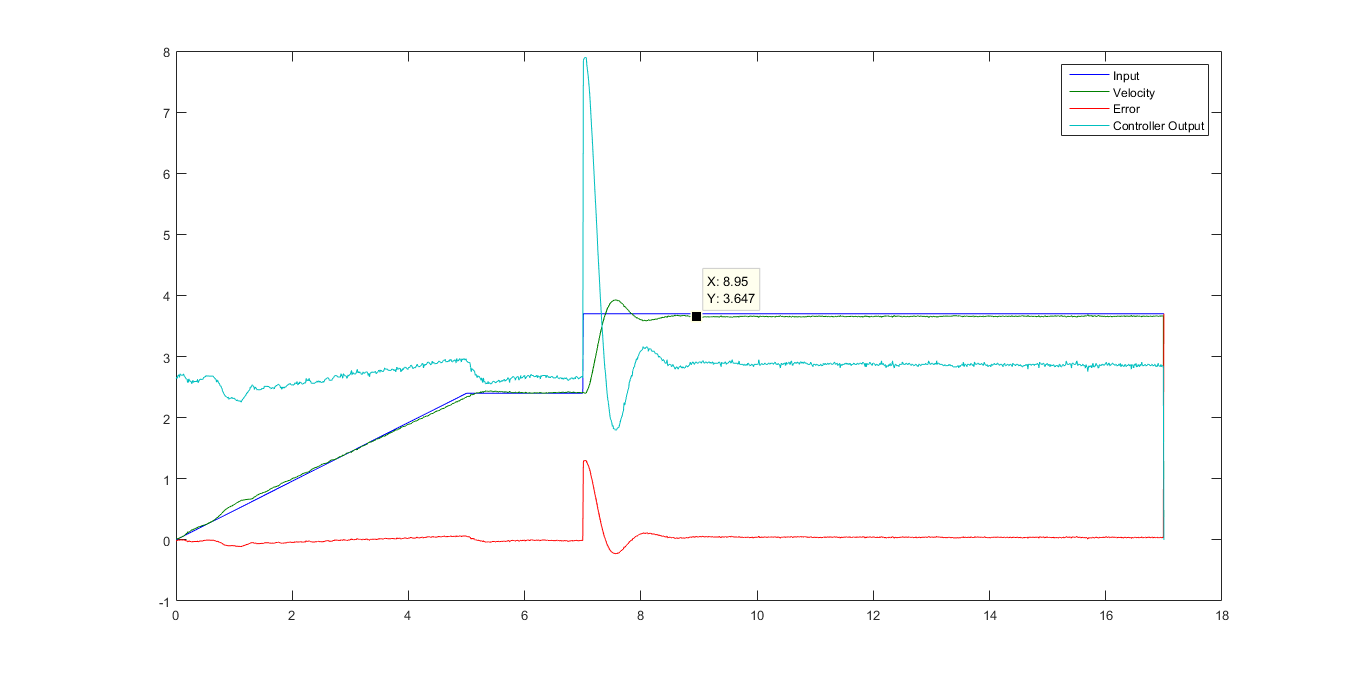
\includegraphics[width = \textwidth]{pics/RM_K4.png}
\caption{Response of the left motor behaviour for $K = 4$ to the blue curve as input.}
\label{fig:RM_K4}
\end{figure}


\section{Conclusions}
A proportional controller was chosen to have a fast response to disturbances. The fact that there can be a steady state error is less important since this loop is controlled by another feedback loop. The outer loop will be able to compensate for the steady state error.

As we did for the other motor, the behaviour was identified using a step between two operating points. Starting from the obtained transfer function some simulations and experiments were done with proportional control. Finally a gain of $K = 3$ was selected. 


\chapter{Modelling and Control of the Traction}
\label{chap:traction}
\section{Modelling of the Traction of the Metallic Strip}
As we said in the introduction, we know from a physical intuition that the traction in the metallic strip depends mainly on the difference of speed between the rolls, rather than on each of the speeds individually. For this reason, we only have to determine $G(p)$ as described in figure \ref{fig:tractionInput}, where $\omega_i$ is the speed of a motor, and $t$ is the traction of the metallic strip.
\begin{figure}[htbp]
\centering
\begin{tikzpicture}[auto, node distance=2cm,>=latex']
    % We start by placing the blocks
    \node [sum] (sum) {};
    \node [input, left of = sum, yshift = 1cm] (vr) {};
    \node [input, left of = sum, yshift = -1cm](vl) {};
    \node [sum, right of = sum, xshift = 1cm](addspeedsetpoint){};
    \node [input, below of = addspeedsetpoint](speed0){};
    \node [block, right of = addspeedsetpoint, xshift = 1cm](strip){$G(s)?$};
    \node [sum, right of = strip, xshift = 2cm](addtracsetpoint){};
    \node [input, below of = addtracsetpoint](tracsetpoint){};
    \node [output, right of = addtracsetpoint](trac){};

    % Once the nodes are placed, connecting them is easy.
    \draw [draw,->] (vr) node [yshift = 3mm]{$\omega_R$} -| node [pos = 0.9]{$+$} (sum);
    \draw [draw,->] (vl) node [yshift = 3mm]{$\omega_L$} -| node [pos = 0.9]{$-$} (sum);
    \draw [draw,->] (sum) -- node {$\Delta_\omega$} node[pos = 0.9]{$+$}  (addspeedsetpoint);
    \draw [draw,->] (speed0) -- node{${\Delta_\omega}_0$} node [pos = 0.9]{$-$} (addspeedsetpoint);
    \draw [draw,->]  (addspeedsetpoint) -- node{${\tilde{\Delta_\omega}}$} (strip);
    \draw [draw,->] (strip) -- node {$\tilde{f}$} node[pos = 0.9]{$+$} (addtracsetpoint);
    \draw [draw,->] (tracsetpoint) -- node {$f_0$} node[pos = 0.9]{$+$} (addtracsetpoint);
    \draw [draw,->] (addtracsetpoint) -- node {$f$} (trac);

\end{tikzpicture}
\caption{\label{fig:tractionInput}Simple gray-box model of the traction of the metallic strip}
\end{figure}

Furthermore, we also know that $G(s)$ should contain a close-to-perfect integrator. Indeed, if we increase $\Delta_\omega$ slightly from the setpoint ${\Delta_\omega}_0$, we expect the tension in the metallic strip to rise indefinitely until breakage. This is also confirmed by the experience: we observe that the system's response to a real world pulse is really close to a step, as showed in figure \ref{fig:tracImpulseResponse}.

\begin{figure}[htbp]
\centering
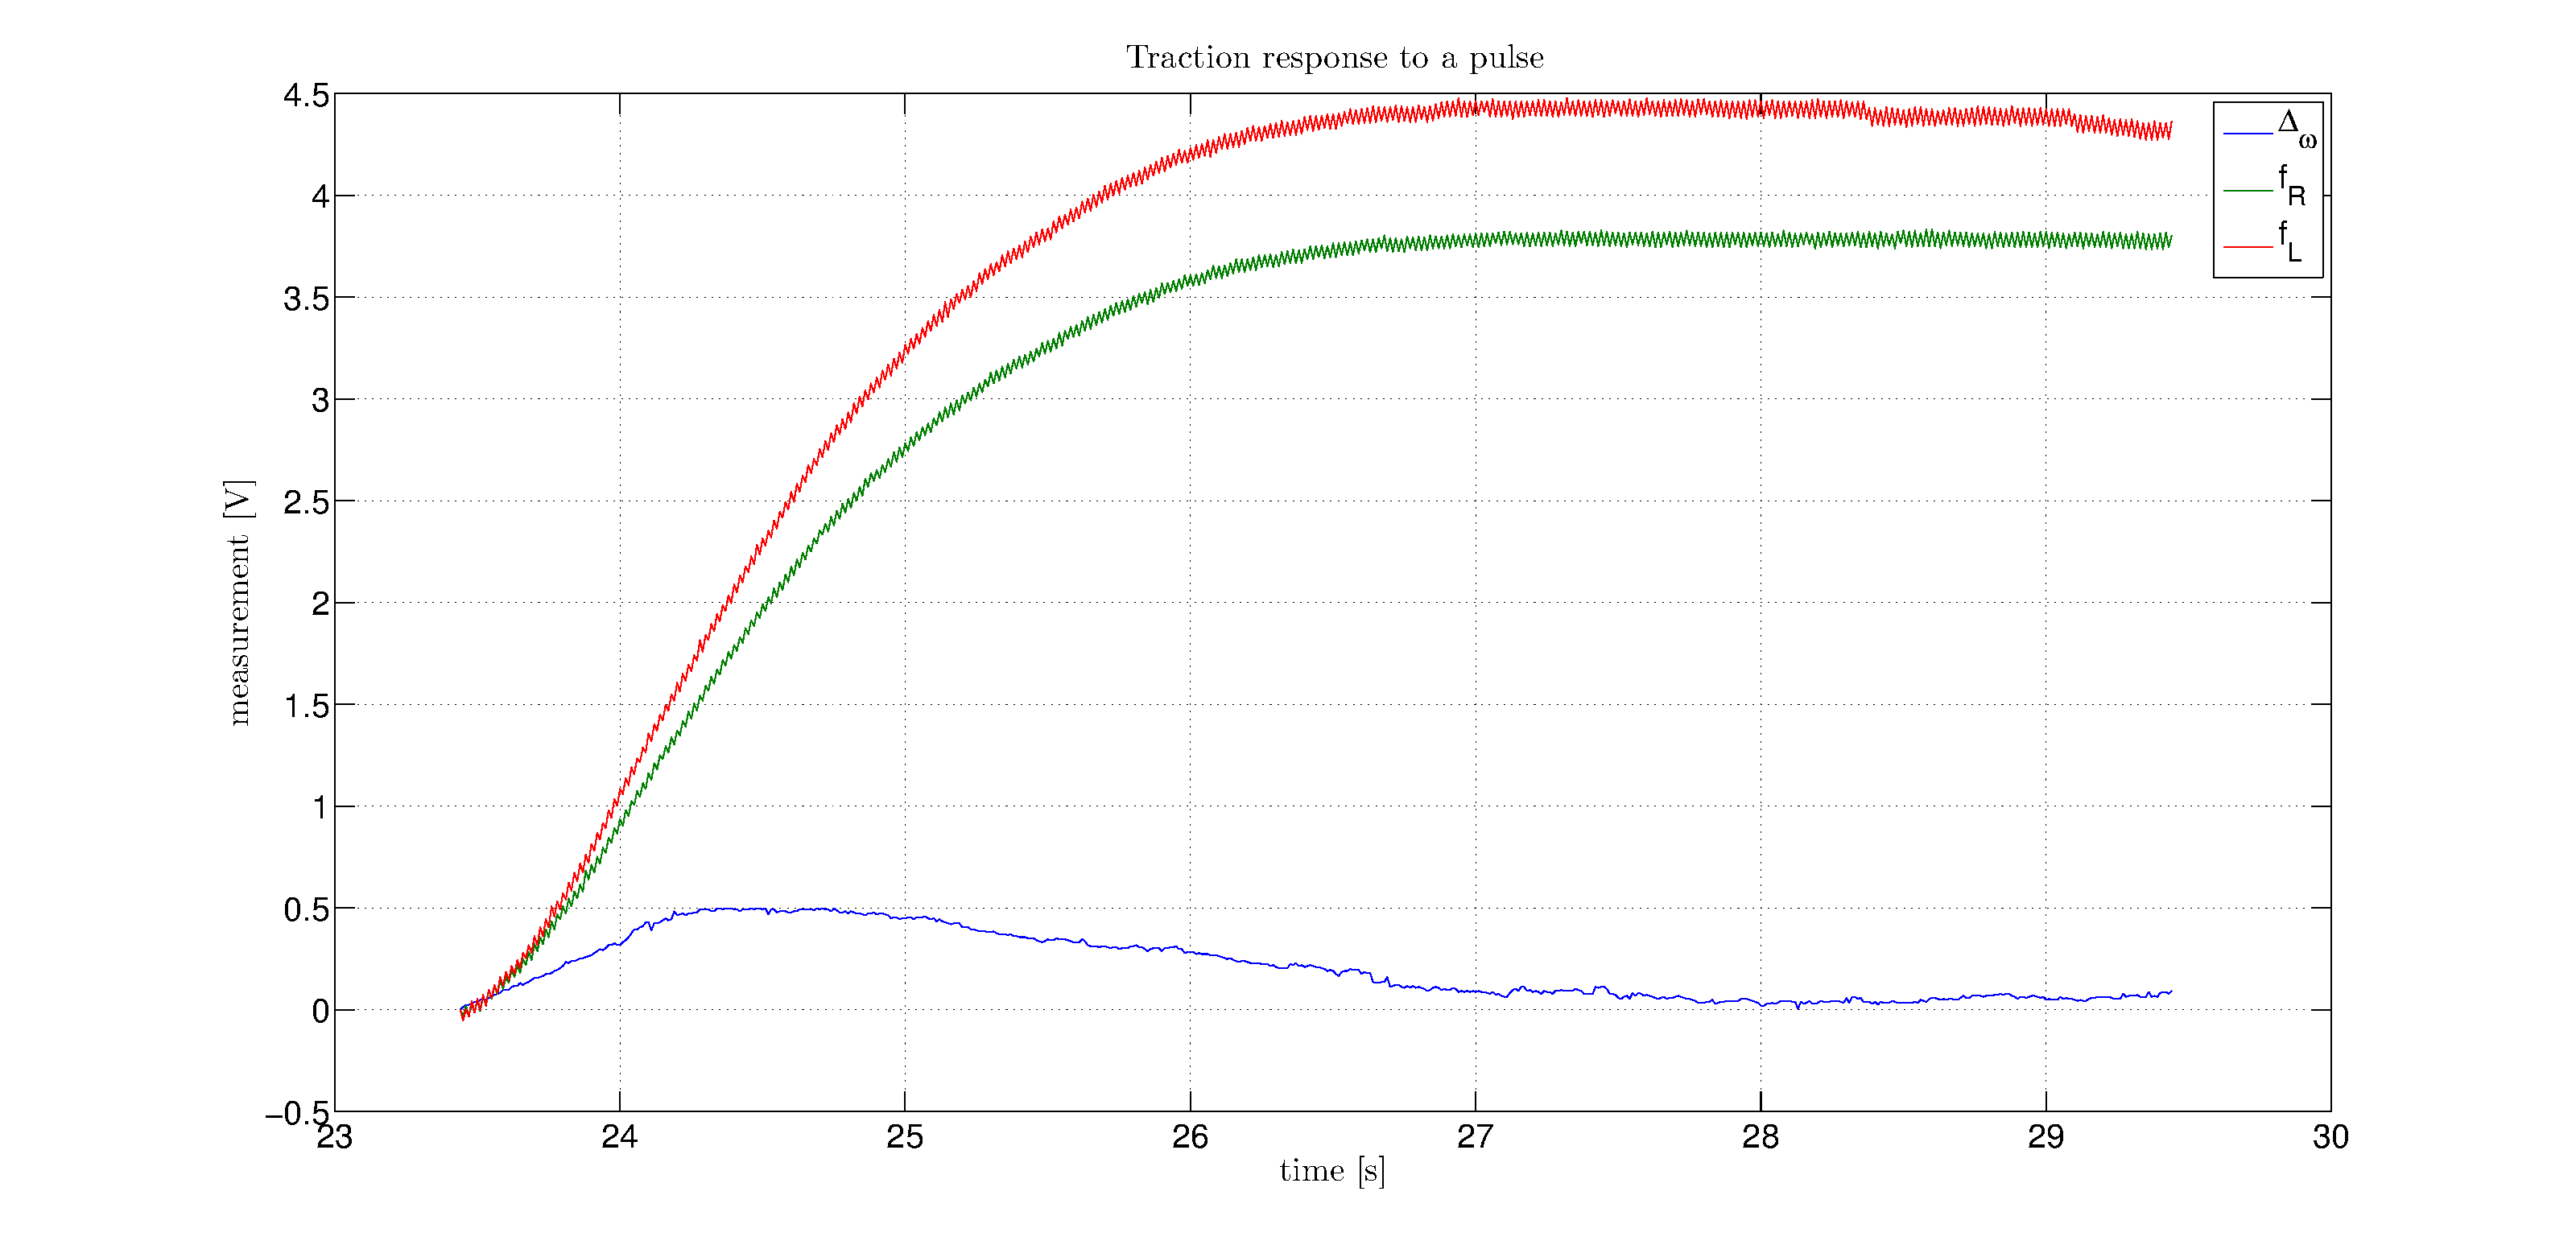
\includegraphics[width = \textwidth]{tractionPulse.pdf}
\caption{Traction response to a real world pulse\label{fig:tracImpulseResponse}}
\end{figure}

Finally, we also see that a second order numerical approximation of the dynamics always yields a pole that is very close to zero. However this leads the rest of the optimisation problem to be badly conditioned. This means that the second pole is not reliably placed, and that the final result does not fit the real response accurately. Moreover, a system with zero very far from the origin takes a really long time to simulate with simulink.

To solve this, we refine our gray-box approximation by introducing an integrator in the system, computing its response to $\tilde{\Delta_\omega}(t)$ and trying to determine the rest of the dynamics based on this new input and the observed response, as shown in figure \ref{fig:tractionGrayBox}, where $\frac{1}{s}H(s) = G(s)$. In the figure, we also utilized the fact that only $\omega_L$ contributes to $\tilde{\Delta_\omega}$, since the master velocity is chosen steady.
\begin{figure}[htbp]
\centering
\begin{tikzpicture}[auto, node distance=2cm,>=latex']
    % We start by placing the blocks
    \node [input](input){};
    \node [square, right of = input, xshift = 1cm](integrator){$\frac{1}{s}$};
    \node [block, right of = integrator, xshift = 2.5cm](strip){$H(s)?$};
    \node [output, right of = strip](trac){};

    % Once the nodes are placed, connecting them is easy.
    \draw [draw,->]  (input) -- node{${\tilde{\omega_L}}$} (integrator);
    \draw [draw,->]  (integrator) -- node{${\int^t_0\tilde{\omega_L}}dt$} (strip);
    \draw [draw,->] (strip) -- node {$\tilde{f}$} (trac);
\end{tikzpicture}
\caption{\label{fig:tractionInput}Gray-box model of the traction of the metallic strip\label{fig:tractionGrayBox}}
\end{figure}

Fitting a simple first order transfer function to $H(s)$ is not easy because the dynamics between $\frac{\tilde{\Omega_L}}{s}$ and $F_R(s)$ is very fast, as shown in figure \ref{fig:tractionPulseStep}. This leads to very large poles which are not well approximated and difficult to simulate, as we experienced already.
\begin{figure}[htbp]
\centering
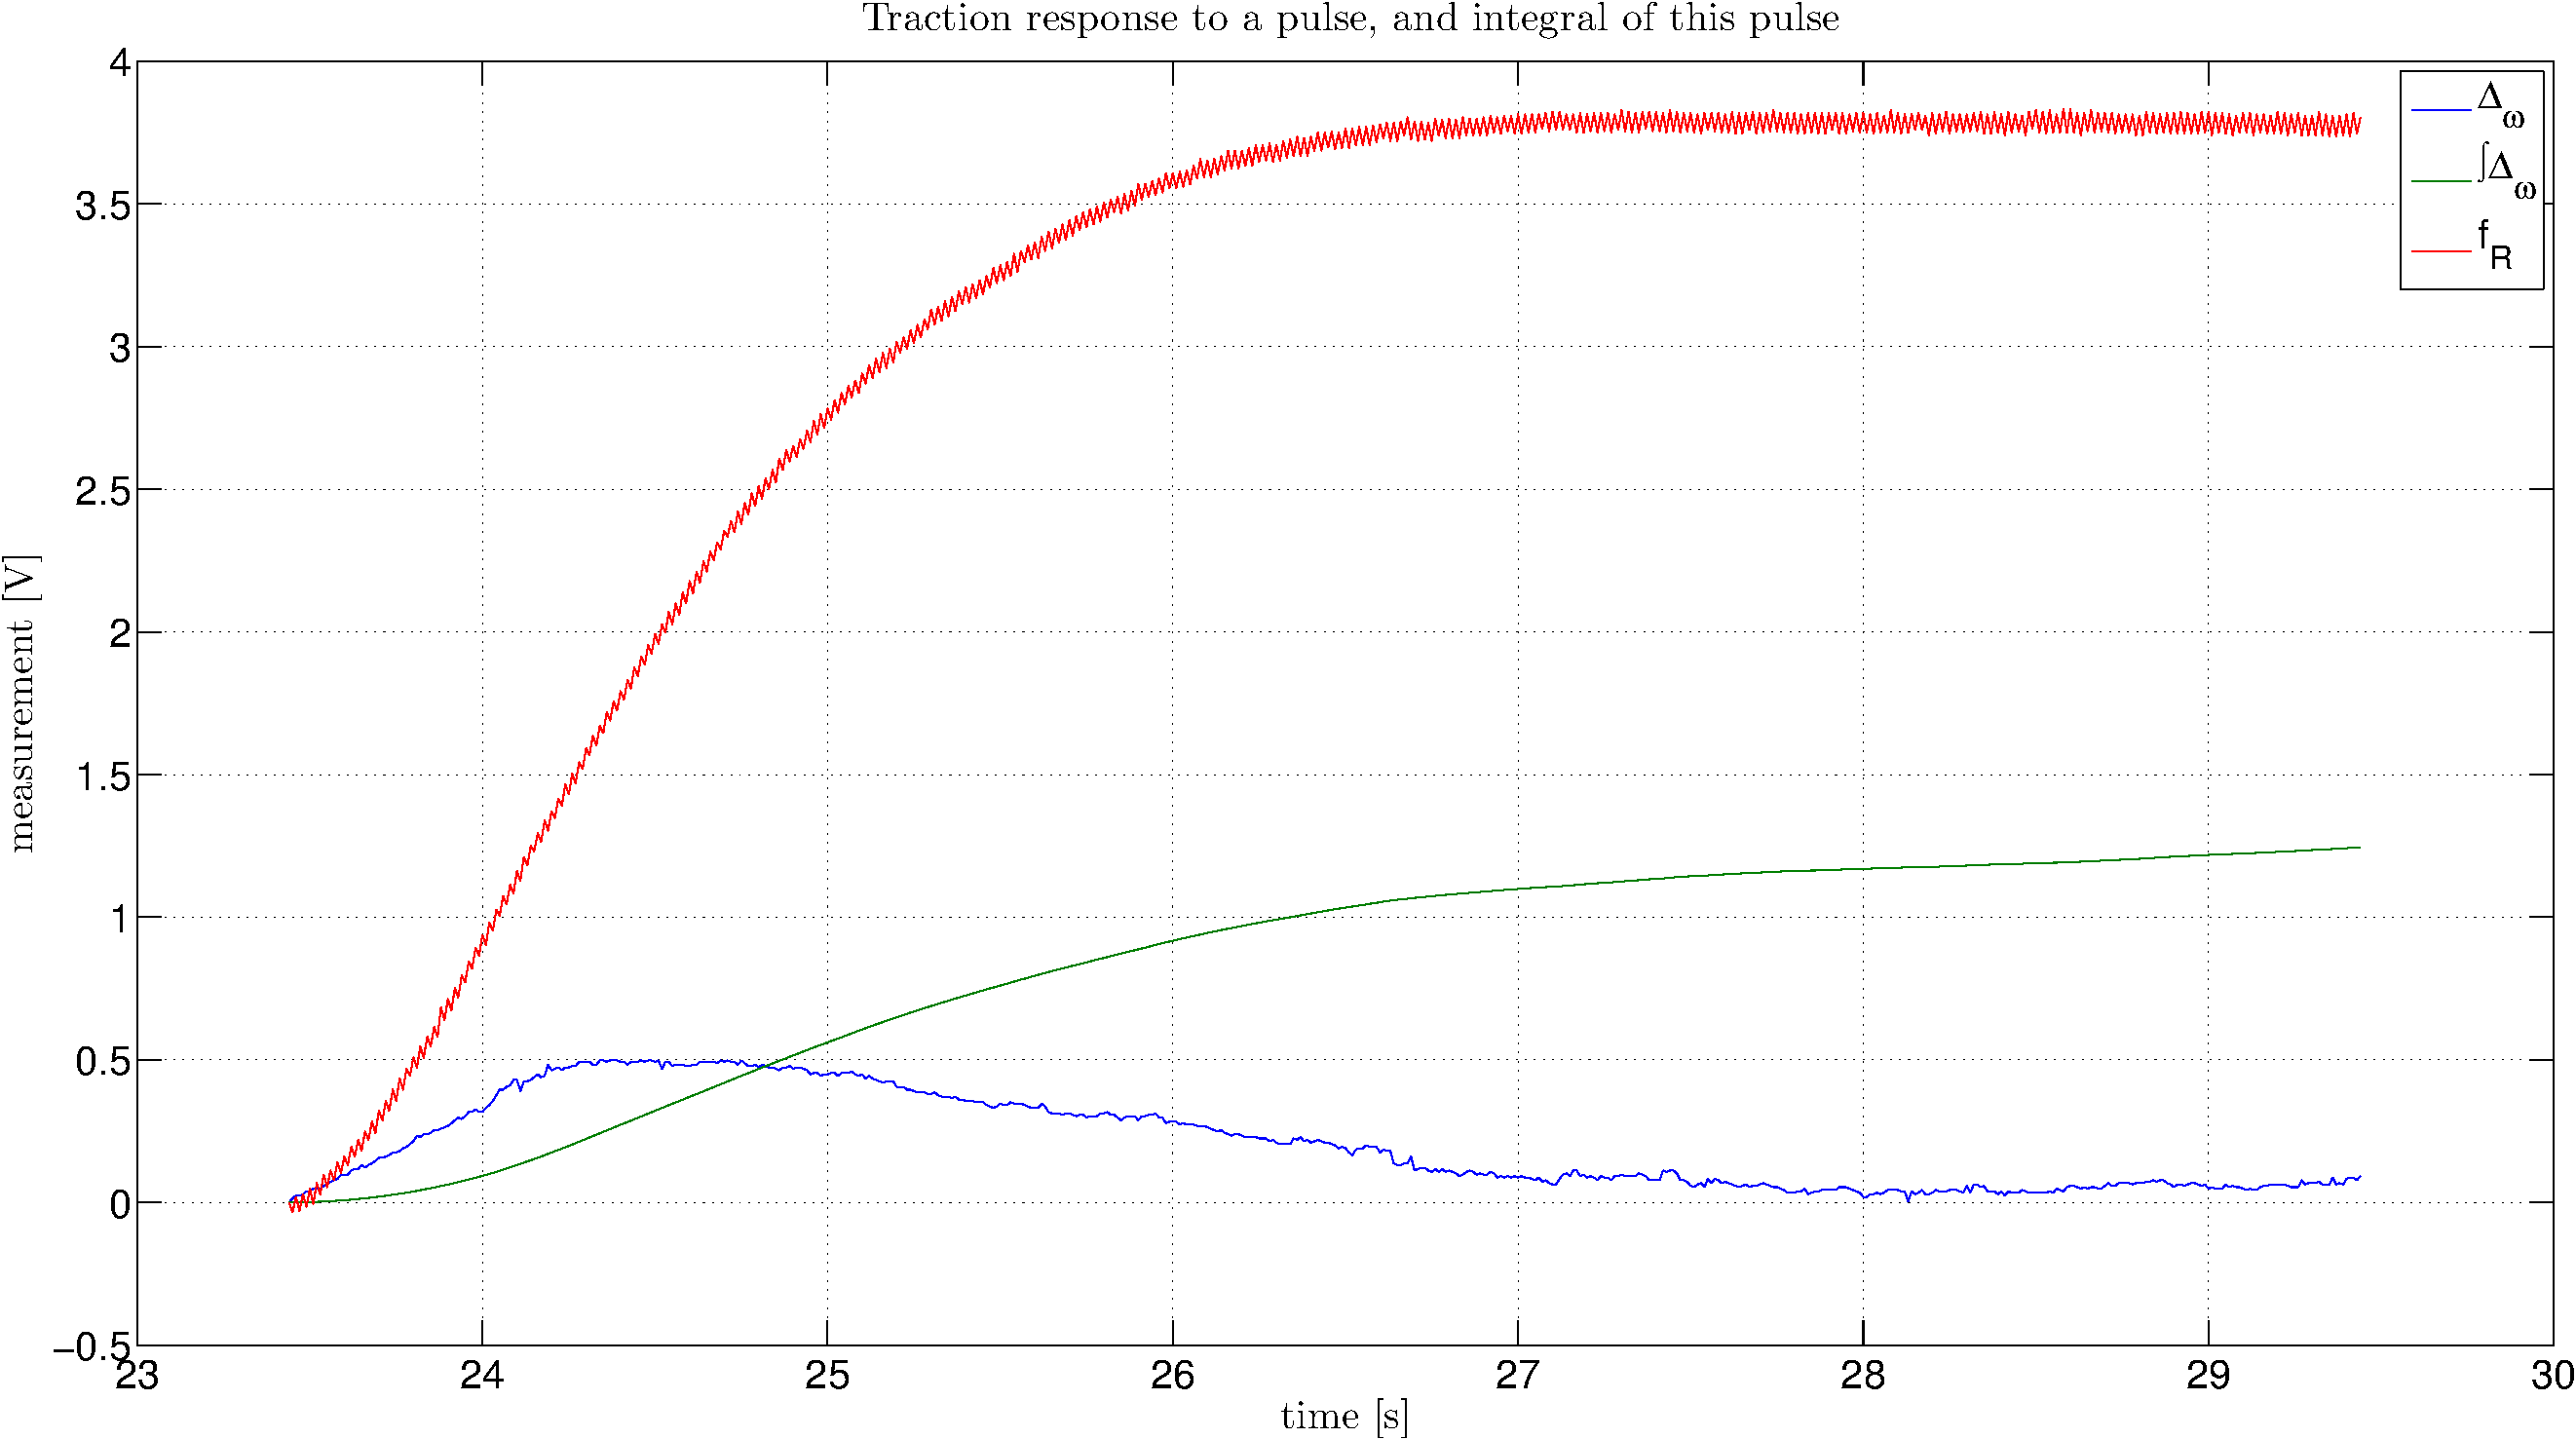
\includegraphics[width = \textwidth]{tractionPulseStep.pdf}
\caption{Right traction response to a pulse and output of the intermediate integrator\label{fig:tractionPulseStep}}
\end{figure}

To solve this, we tried to fit $H(s)$ with a transfer function of the form $K\frac{s-z_0}{s-p_0}$, because the introduction of a zero speeds up a step response, which would bring $p_0$ reasonably closer to the origin. The result is shown in figure \ref{fig:tracFit}, where we see that the following transfer function seems to fit the experience very well.
\[H(s) = 13.096\frac{s+0.9221}{s(s+4.063)}\]
\begin{figure}[htbp]
\centering
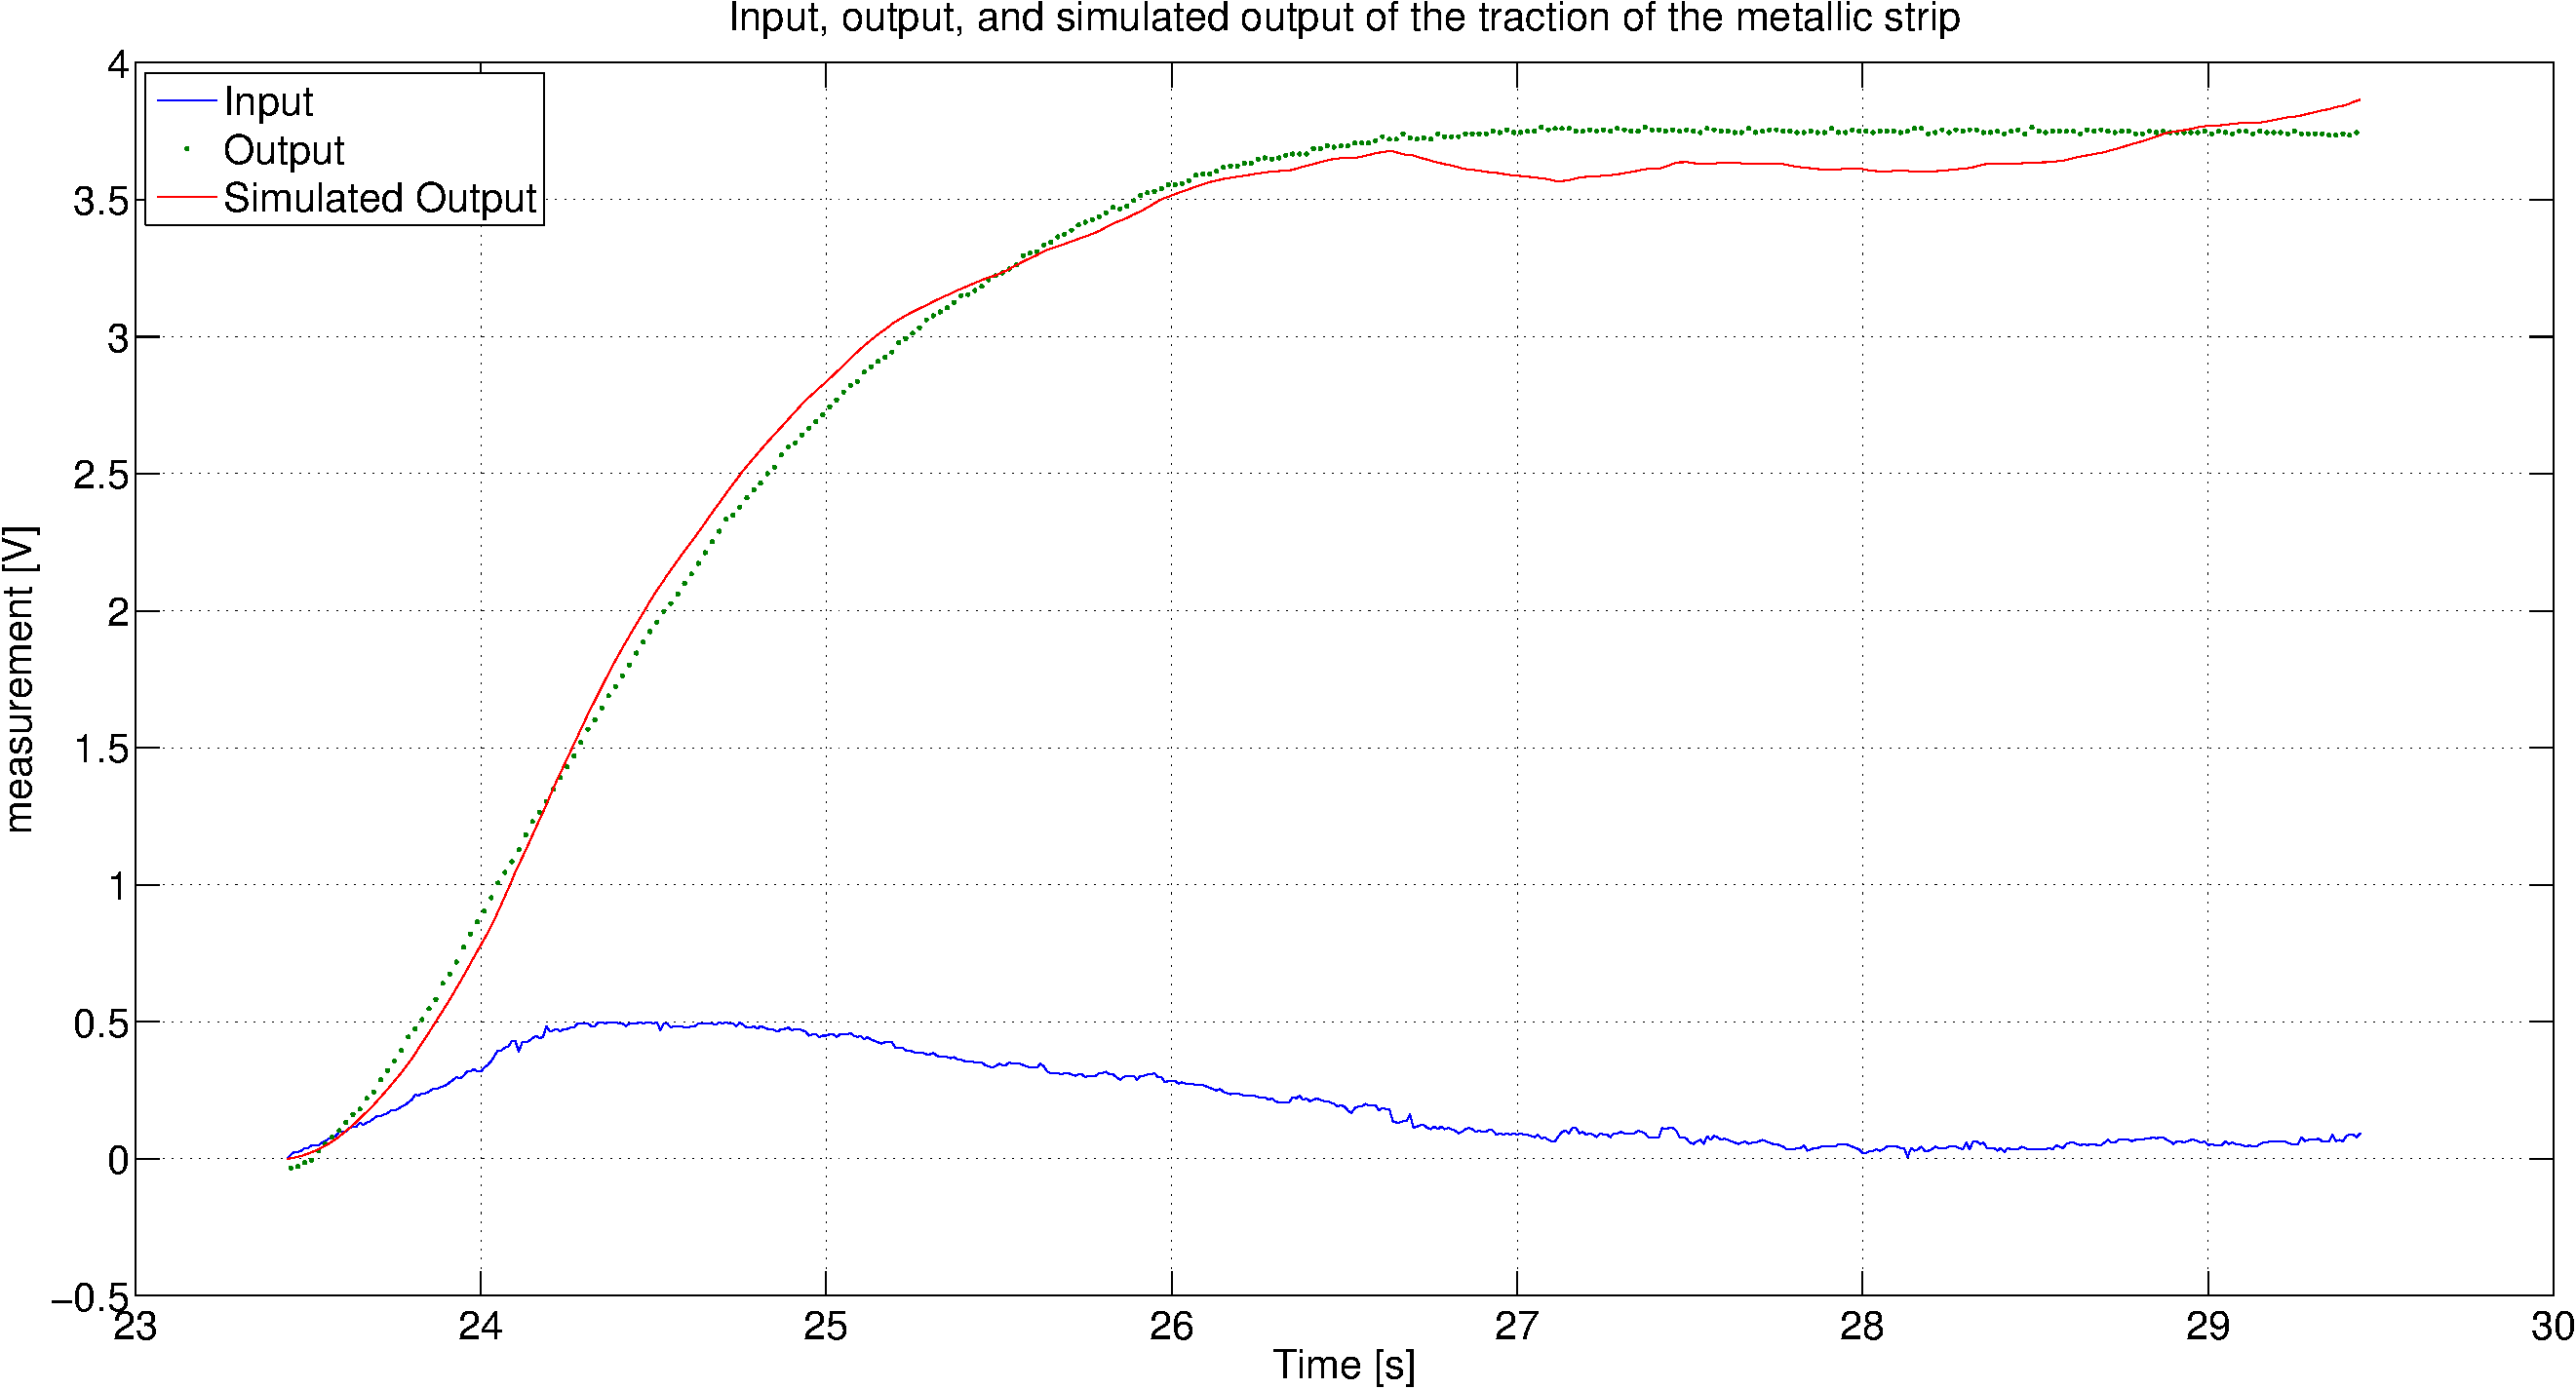
\includegraphics[width = \textwidth]{tracFit.pdf}
\caption{Input, output, and simulated output of the traction of the metallic strip\label{fig:tracFit}}
\end{figure}



\chapter{Thickness control}
\label{chap:thickness}
In this section some considerations will be made about the more advanced objective. Since it is not attainable in the course of five lab sessions only some theoretical reflections will be made. The more advanced objective was to be able to control the output thickness of the metallic strip.

\section{Workings of the Complete Rolling Mill Plant}
The full workings of the mill are as follows: one motor unwinds the metal strip from a spool. The metal strip passes between two cylinders driven by a second motor. The metal is compressed between these too cylinders and is subsequently wound up by the third motor. The thickness is mainly controlled by the distance between the two rolls but also depends on the other parameters of the plant in a non linear way. This distance can be controlled manually by a crank.

We have three motors as actuators, one manual setting for the middle rolls spacing, and multiple sensors:
\begin{itemize}
\item Thickness sensor before/after the rolls
\item Traction sensor before/after the rolls
\item Velocity sensors for each of the motors
\item Rolling force sensor
\end{itemize}
The technical reason the objective is not attainable is that there are not enough DAC ports to control every motor independently. In terms of required research and time, this project would also be more fitted as a master thesis. Still, in the following, we will present a possible approach to try to control the thickness of the metallic strip.

\section{Controller considerations}
First, the plant has to be biased around a setpoint depending on the desired output thickness. The bias parameters are the master speed, which is now the speed of the middle pair of rolls, the spacing between the middle rolls and the traction left and right of the middle pair of rolls. For a given desired output thickness, those biasing parameters can be found in a table describing the rolling mill. Around this setpoint, the thickness has to be controlled using small signal variations of the left and right traction.

To control the thickness, one should use a cascade controller on top of the traction controller we already designed during this report. However, the existing controller must be adapted to use the middle motor as master motor, and duplicated in order to independently control the left and right traction.

From there on, one has to see if it is possible to again simplify the controlling scheme by fixing a traction on a steady value and only controlling the other one around a master value. A worse case would be that both tractions have to be dynamically controlled simultaneously in order to ensure the plant works properly. In the worst case, the traction variations needed to control the thickness are so large that the speed setpoint has to be changed during the operation. In that case, the controller has to implement a lookup table in order to control the non linear parameters.

With such a setup, it should be at least possible to control the thickness of the metallic strip around a constant reference. As we showed, tracking a dynamic reference would be an even more advanced requirement due to the heavy non linearity of the plant. However, there are already ports available to control the spacing of the middle rolls while in operation rather than using a manual crank. Using this extra dynamic input should make thickness reference tracking possible, using lookup tables and the work presented in this report.


\appendix
\chapter{Controller code}
\label{chap:code}
\setcounter{page}{1}
\pagenumbering{alph}
\begin{matlabcode}
%controller.m
function [time, reference, output, input, innerTractionRefArray, rSpeedRefArray] = controller()

  %%%%%%%%%%%%%%%%%%%%%%%%%%%%%%%%%%%%%%%%%%%%%%%%%%%%%%%%%%%%%%%%%%%%%%%%%%
  %Control System Design Lab: Overall Controller Loop
  %%%%%%%%%%%%%%%%%%%%%%%%%%%%%%%%%%%%%%%%%%%%%%%%%%%%%%%%%%%%%%%%%%%%%%%%%%
  %%
  %%%%%%%%%%%%%%%%%%%%%%%%%%%%%%%%%%%%%%%%%%%%%%%%%%%%%%%%%%%%%%%%%%%%%%%%%%
  %Setup
  %%%%%%%%%%%%%%%%%%%%%%%%%%%%%%%%%%%%%%%%%%%%%%%%%%%%%%%%%%%%%%%%%%%%%%%%%%

  T_S = 0.01;%Set the sampling time.


  function [nSamples, time, reference, output, input] = referenceGenerator()
    %REF(1,:) = traction
    %REF(2,:) = master speed

    %traction
    EXP_LENGTH = 50;%sec
    TRACTION_REF = 3;
    TRAC_SETUP_TIME = 8;

    tracRamp = 0:T_S*TRACTION_REF/TRAC_SETUP_TIME:TRACTION_REF;
    reference(1,:) = [tracRamp TRACTION_REF*ones(1, EXP_LENGTH/T_S - length(tracRamp))];

    %master
    SETUP_TIME = 8;%seconds
    SETUP_POINT = 2;%V Left Motor

    ramp = 0:T_S*SETUP_POINT/SETUP_TIME:SETUP_POINT;
    rampLength = length(ramp);

    reference(2,:) = [ramp ones(1,length(reference(1,:))-rampLength)*SETUP_POINT];

    nSamples = length(reference);
    time=0:T_S:(nSamples-1)*T_S;
    output = zeros(2, nSamples);
    input = zeros(8, nSamples);
  end
\end{matlabcode}
\clearpage
\begin{matlabcode}
  %%
  %%%%%%%%%%%%%%%%%%%%%%%%%%%%%%%%%%%%%%%%%%%%%%%%%%%%%%%%%%%%%%%%%%%%%%%%%%
  %Controllers
  %%%%%%%%%%%%%%%%%%%%%%%%%%%%%%%%%%%%%%%%%%%%%%%%%%%%%%%%%%%%%%%%%%%%%%%%%%

  function current = lmController(speedRef, measuredSpeed)
    if speedRef < 0
      FRICTION_COMPENSATOR  = -2.7;
    else
      FRICTION_COMPENSATOR  = 2.7;
    end
    KP = 2;
    KI = KP/3.642;

    persistent errorIntegral;
    if isempty(errorIntegral)
      errorIntegral = 0;
    end

    error = speedRef - measuredSpeed;
    errorIntegral = errorIntegral + error*T_S;

    current = FRICTION_COMPENSATOR + KP*error + KI*errorIntegral;
  end

  function current = rmController(speedRef, measuredSpeed)
    if speedRef < 0
      FRICTION_COMPENSATOR  = -2.1;
    else
      FRICTION_COMPENSATOR  = 2.1;
    end
    KP = 3;

    error = speedRef - measuredSpeed;
    current = FRICTION_COMPENSATOR + KP*error;
  end

  function speedRef = innerLoopSpeed(traction, innerTractionRef)
    K = -0.123;
    speedRef = K*(innerTractionRef-traction);
  end

  function innerTractionRef = outerLoopTraction(traction, tractionRef)
    persistent errorIntegral;
    if isempty(errorIntegral)
      errorIntegral = 0;
    end
    K = 2;
    ZERO = 1.9;
    KI = ZERO*K;
    error = tractionRef - traction;
    errorIntegral = errorIntegral + error*T_S;
    innerTractionRef = K*(error) + KI*errorIntegral;
  end

\end{matlabcode}
\clearpage
\begin{matlabcode}
  %%
  %%%%%%%%%%%%%%%%%%%%%%%%%%%%%%%%%%%%%%%%%%%%%%%%%%%%%%%%%%%%%%%%%%%%%%%%%%
  %Main Loop
  %%%%%%%%%%%%%%%%%%%%%%%%%%%%%%%%%%%%%%%%%%%%%%%%%%%%%%%%%%%%%%%%%%%%%%%%%%
  [nSamples, time, reference, output, input] = referenceGenerator();
  %precompute the reference and generate arrays of according size
  innerTractionRefArray = zeros(1,nSamples);
  rSpeedRefArray = zeros(1,nSamples);
  i=1;
  while i < nSamples
    tic %Begins the first strike of the clock.
    [input(1,i), input(2,i), input(3,i), input(4,i), input(5,i), ...
      input(6,i), input(7,i), input(8,i)]  = anain; %Acquisition of the measurements.

    rmVelocity = input(5,i); %saving the inputs in a variable for ease of working
    lmVelocity = input(4,i);
    lTraction = input(3,i);
    rTraction = input(2,i);

    if(lTraction > 6 || rTraction > 6) % safety measures if traction is to high
      lmCurrent = 0;
      rmCurrent = 0;
      i = nSamples + 1;
    else
      lmCurrent = lmController(reference(2,i), lmVelocity);

      %Cascade loops
      innerTractionRef = outerLoopTraction(rTraction, reference(1,i));
      rSpeedRef = innerLoopSpeed(rTraction, innerTractionRef);
      rmCurrent = rmController(rSpeedRef, rmVelocity);
      innerTractionRefArray(i) = innerTractionRef;
      rSpeedRefArray(i) = rSpeedRef;
    end

    output(2,i) = rmCurrent;
    output(1,i) = lmCurrent;
    anaout(lmCurrent, rmCurrent);

    if toc > T_S
      disp('Sampling time too small');%Test if the sampling time is too small.
    else
      while toc <= T_S
        %Does nothing until the second strike of the clock reaches the sampling time set.
      end
    end
    i=i+1;
  end
end
\end{matlabcode}
\clearpage
\begin{matlabcode}
%main.m
openinout;
[time, reference, output, input, innerTractionRef, rSpeedRef] = controller();
anaout(0,0);
closeinout;
%%
%%%%%%%%%%%%%%%%%%%%%%%%%%%%%%%%%%%%%%%%%%%%%%%%%%%%%%%%%%%%%%%%%%%%%%%%%%
%Plots
%%%%%%%%%%%%%%%%%%%%%%%%%%%%%%%%%%%%%%%%%%%%%%%%%%%%%%%%%%%%%%%%%%%%%%%%%%
figure %Open a new window for plot.
plot(time,reference(1,:), time, input(2,:), time,...
  input(4,:), time, input(5,:), time, rSpeedRef); %Plot the experiment (input and output).
legend('traction reference','traction','master speed',...
  'slave speed', 'slave speed reference');
title('Reference and output values')
xlabel('Time [s]');ylabel('Measurement [V]');

figure;
plot(time, output(1,:), time, output(2,:));
legend('Master motor current', 'Slave motor current');
title('Actuators input')
xlabel('Time [s]');ylabel('Value [V]');
\end{matlabcode}


\hypersetup{allcolors = black}
\listoffigures
\addcontentsline{toc}{chapter}{\listfigurename}

\end{document}
